\documentclass[a4paper,12pt]{article}
\usepackage{standalone}
\usepackage[a4paper, top=0.8in, bottom=0.7in, left=0.8in, right=0.8in]{geometry}
\usepackage{amsmath}
\usepackage{hyperref}
\usepackage{amsfonts}
\usepackage{latexsym}
\usepackage{graphicx}
\usepackage{fancyhdr}
\usepackage{enumitem}
\usepackage{setspace}
\usepackage{tcolorbox}
\usepackage{tikz}
\usepackage{multicol}
\usepackage[defaultfam,tabular,lining]{montserrat} % Font settings for Montserrat

\usepackage{xcolor}  % To use colors
\hypersetup{
    colorlinks=true,   % Activate colored links
    linkcolor=blue,    % Link color for internal links
    urlcolor=blue,     % Link color for URLs
    filecolor=blue,    % Link color for file links
    menucolor=blue,    % Link color for menus
}

\sloppy

\title{}
\date{}
\hyphenpenalty=10000
\exhyphenpenalty=10000

\setlength{\parindent}{0pt}
\pagestyle{fancy}

\setlength{\headheight}{27.11148pt}
\addtolength{\topmargin}{-15.11148pt}

\fancyhf{}
\fancyhead[L]{\textbf{Curriculum D TWB}}
\fancyhead[R]{\includegraphics[width=0.8cm]{Round Logo.png}} % Placeholder for logo
\fancyfoot[C]{\footnotesize \textcopyright{} Study Smart Tutors}
\fancyfoot[R]{\thepage}  % Page number in bottom right corner
\fancyfoot[L]{\hyperlink{toc}{Back to Contents}} % Clickable link in bottom left to TOC

\sloppy

% Define a new command for the level letter
\newcommand{\levelLetter}{D}  % Change this letter to update throughout the document

%%%%%%%%%%%%%%%%%%%%%%%%%%%%%%%%%%%%%

\begin{document}

% Title Page
\input{Tutoring Cover Pages/Math Curriculum Materials Cover Pages/Instr.Curriculum D Math.tex} % Include the title page content here
title page content here
\pagenumbering{gobble}
\hypertarget{toc}{}  % Mark the TOC as a hyperlink target
% Table of Contents
\tableofcontents
\newpage

% Restart page numbering from 1 after TOC
\pagenumbering{arabic}
\pagestyle{fancy}  % Re-enable fancy headers/footers

% Guided Lesson and Answer Key for 3.OA.A.1, 3.OA.A.3
\newpage
\section{3.OA.A.1, 3.OA.A.3 Guided Lesson (Instructor Version)}
\documentclass[12pt]{article}
\usepackage[a4paper, top=0.8in, bottom=0.7in, left=0.8in, right=0.8in]{geometry}
\usepackage{amsmath, amsfonts, latexsym, graphicx, fancyhdr, enumitem, setspace, tcolorbox, textcomp, xcolor}
\usepackage[defaultfam,tabular,lining]{montserrat} % Font settings for Montserrat

\setlength{\parindent}{0pt}
\pagestyle{fancy}

\setlength{\headheight}{27.11148pt}
\addtolength{\topmargin}{-15.11148pt}

\fancyhf{}
%\fancyhead[L]{\textbf{Standard(s): 3.OA.A.1, 3.OA.A.3}} % Example standards
\fancyhead[R]{\includegraphics[width=0.8cm]{Round Logo.png}} % Placeholder for logo
\fancyfoot[C]{\footnotesize \textcopyright Study Smart Tutors}

\title{}
\date{}
\hyphenpenalty=10000
\exhyphenpenalty=10000

\begin{document}

\subsection*{Guided Lesson: Understanding Multiplication and Division}
\onehalfspacing

% Guided Practice
\begin{tcolorbox}[colframe=black!60, colback=white, 
coltitle=black, colbacktitle=black!15, fonttitle=\bfseries\Large, 
title=Guided Practice, halign title=center, left=10pt, right=10pt, top=10pt, bottom=80pt]
\textbf{Solve the following problems with teacher support:}
\begin{enumerate}[itemsep=5em] % Increased spacing for student work
    \item A teacher has 5 boxes of pencils, with 6 pencils in each box. How many pencils are there in total? (Hint: Use multiplication.)
    \\ \textcolor{red}{Solution: $5 \times 6 = 30$ pencils.}
    \item Write a multiplication equation for: "There are 7 shelves of books, and each shelf has 12 books."
    \\ \textcolor{red}{Solution: $7 \times 12 = 84$ books.}
    \item A bag contains 30 candies divided equally among 5 friends. How many candies does each friend receive?
    \\ \textcolor{red}{Solution: $30 \div 5 = 6$ candies per friend.}
    \item Draw an array to show $4 \times 3$. How many dots are there in total?
    \\ \textcolor{red}{Solution: An array with 4 rows and 3 columns. Total dots: $4 \times 3 = 12$.}
    \item A student groups 24 apples into 4 equal groups. How many apples are in each group? Show your work using a grouping diagram.
    \\ \textcolor{red}{Solution: $24 \div 4 = 6$ apples per group.}
\end{enumerate}
\end{tcolorbox}

% Independent Practice
\begin{tcolorbox}[colframe=black!60, colback=white, 
coltitle=black, colbacktitle=black!15, fonttitle=\bfseries\Large, 
title=Independent Practice, halign title=center, left=10pt, right=10pt, top=10pt, bottom=60pt]
\textbf{Solve the following problems independently:}
\begin{enumerate}[itemsep=5em] % Increased spacing for student work
    \item A farmer has 8 baskets, each with 9 apples. How many apples does the farmer have in total?
    \\ \textcolor{red}{Solution: $8 \times 9 = 72$ apples.}
    \item A student has 42 marbles and divides them into 7 groups. How many marbles are in each group?
    \\ \textcolor{red}{Solution: $42 \div 7 = 6$ marbles per group.}
    \item Write a division equation for: "A bag of 50 candies is shared equally among 10 children."
    \\ \textcolor{red}{Solution: $50 \div 10 = 5$ candies per child.}
    \item Draw an array to represent $5 \times 6$. How many dots are there?
    \\ \textcolor{red}{Solution: An array with 5 rows and 6 columns. Total dots: $5 \times 6 = 30$.}
    \item A school has 48 desks arranged into 6 rows. How many desks are in each row?
    \\ \textcolor{red}{Solution: $48 \div 6 = 8$ desks per row.}
\end{enumerate}
\end{tcolorbox}

% Exit Ticket
\begin{tcolorbox}[colframe=black!60, colback=white, 
coltitle=black, colbacktitle=black!15, fonttitle=\bfseries\Large, 
title=Exit Ticket, halign title=center, left=10pt, right=10pt, top=10pt, bottom=15pt]
\textbf{Answer the following question:}
\begin{itemize}
    \item How are multiplication and division related? Provide an example. Use a visual representation to support your explanation.
    \\ \textcolor{red}{Solution: Multiplication and division are inverse operations. Example: $4 \times 5 = 20$ and $20 \div 5 = 4$. Visual: An array with 4 rows and 5 columns shows 20 dots, which can be split into equal groups.}
\end{itemize}
\vspace{5cm}
\end{tcolorbox}

\end{document}


\newpage
\section{3.OA.A.1, 3.OA.A.3 Problem Set Answer Key}
\input{Grade 3/PS Answer Keys/Generic.KEY.3.OA.A.1, 3.OA.A.3.tex}

% Guided Lesson and Answer Key for 3.OA.A.4
\newpage
\section{3.OA.A.4 Guided Lesson (Instructor Version)}
\input{Grade 3/Grade 3 Guided Lesson/Generic.3.OA.A.4.GL.Instructor Version.tex}

\newpage
\section{3.OA.A.4 Problem Set Answer Key}
\documentclass[11pt]{article}
\usepackage[a4paper, top=0.8in, bottom=0.7in, left=0.8in, right=0.8in]{geometry}
\usepackage{amsmath}
\usepackage{amsfonts}
\usepackage{graphicx}
\usepackage{fancyhdr}
\usepackage{tcolorbox}
\usepackage{enumitem}
\usepackage{setspace}
\usepackage[defaultfam,tabular,lining]{montserrat}
\usepackage{xcolor}

\setlength{\parindent}{0pt}
\pagestyle{fancy}

\setlength{\headheight}{27.11148pt}
\addtolength{\topmargin}{-15.11148pt}

\fancyhf{}
%\fancyhead[L]{\textbf{3.OA.A.4: Multiplication and Division Problem Solving - Answer Key}}
\fancyhead[R]{\includegraphics[width=0.8cm]{Round Logo.png}}
\fancyfoot[C]{\footnotesize © Study Smart Tutors}

\sloppy

\title{}
\date{}
\hyphenpenalty=10000
\exhyphenpenalty=10000

\begin{document}

\subsection*{Problem Set: Multiplication and Division Problem Solving - Answer Key}
\onehalfspacing

% Learning Objective Box
\begin{tcolorbox}[colframe=black!40, colback=gray!5, 
coltitle=black, colbacktitle=black!20, fonttitle=\bfseries\Large, 
title=Learning Objective, halign title=center, left=5pt, right=5pt, top=5pt, bottom=15pt]
\textbf{Objective:} Solve multiplication and division problems involving unknown products, group sizes, and numbers of groups using equal groups, arrays, and comparison situations.
\end{tcolorbox}

% Exercises Box
\begin{tcolorbox}[colframe=black!60, colback=white, 
coltitle=black, colbacktitle=black!15, fonttitle=\bfseries\Large, 
title=Exercises, halign title=center, left=10pt, right=10pt, top=10pt, bottom=60pt]
\textbf{Find the missing number in each problem below:}
\begin{enumerate}[itemsep=2em]
    \item \(8 \times \_\_\_ = 56\)\\
    \textcolor{red}{\textbf{Solution:} \(56 \div 8 = 7\). The missing number is \(7\).}

    \item \(6 \times \_\_\_ = 42\)\\
    \textcolor{red}{\textbf{Solution:} \(42 \div 6 = 7\). The missing number is \(7\).}

    \item \(45 \div \_\_\_ = 9\)\\
    \textcolor{red}{\textbf{Solution:} \(45 \div 9 = 5\). The missing number is \(5\).}

    \item \(\_\_\_ \times 4 = 20\)\\
    \textcolor{red}{\textbf{Solution:} \(20 \div 4 = 5\). The missing number is \(5\).}

    \item \(15 \div \_\_\_ = 5\)\\
    \textcolor{red}{\textbf{Solution:} \(15 \div 5 = 3\). The missing number is \(3\).}

    \item \(3 \times (\_\_\_ + 5) = 27\)\\
    \textcolor{red}{\textbf{Solution:} \(27 \div 3 = 9\), so \((\_\_\_ + 5) = 9\). Subtract \(5\): \(\_\_\_ = 4\). The missing number is \(4\).}

    \item \(\_\_\_ \times 5 = 35\)\\
    \textcolor{red}{\textbf{Solution:} \(35 \div 5 = 7\). The missing number is \(7\).}

    \item \(12 \div \_\_\_ + 6 = 9\)\\
    \textcolor{red}{\textbf{Solution:} \(9 - 6 = 3\), so \(12 \div \_\_\_ = 3\). \(12 \div 3 = 4\). The missing number is \(4\).}

    \item \(9 \div \_\_\_ = 3\)\\
    \textcolor{red}{\textbf{Solution:} \(9 \div 3 = 3\). The missing number is \(3\).}

    \item \(8 \times \_\_\_ = 48\)\\
    \textcolor{red}{\textbf{Solution:} \(48 \div 8 = 6\). The missing number is \(6\).}
\end{enumerate}
\end{tcolorbox}

% Problems Box
\begin{tcolorbox}[colframe=black!60, colback=white, 
coltitle=black, colbacktitle=black!15, fonttitle=\bfseries\Large, 
title=Problems, halign title=center, left=10pt, right=10pt, top=10pt, bottom=60pt]
\begin{enumerate}[start=11, itemsep=3em]
    \item A gardener plants \(5\) rows of flowers with \(8\) flowers in each row. \(3\) flowers in each row are eaten by bugs. Write an equation to find the total number of flowers left.\\
    \textcolor{red}{\textbf{Solution:} Equation: \(5 \times (8 - 3) = 5 \times 5 = 25\). The gardener has \(25\) flowers left.}

    \item A soccer team has \(18\) players. The coach divides them equally into \(3\) teams. Each team gains \(2\) extra players. How many players are now on each team?\\
    \textcolor{red}{\textbf{Solution:} \(18 \div 3 = 6\), then \(6 + 2 = 8\). Each team now has \(8\) players.}

    \item A library has \(120\) books. They are placed equally on \(6\) shelves, and \(12\) books are reserved for a display table. Write and solve an equation to find how many books are on each shelf.\\
    \textcolor{red}{\textbf{Solution:} Equation: \((120 - 12) \div 6 = 108 \div 6 = 18\). Each shelf has \(18\) books.}

    \item A classroom has \(36\) students. The teacher divides them into \(6\) groups. Each group gets \(2\) additional students. How many students are in each group now?\\
    \textcolor{red}{\textbf{Solution:} \(36 \div 6 = 6\), then \(6 + 2 = 8\). Each group now has \(8\) students.}

    \item There are \(12\) chairs in a room. If the chairs are arranged equally into \(4\) rows, how many chairs are in each row? Write and solve an equation.\\
    \textcolor{red}{\textbf{Solution:} Equation: \(12 \div 4 = 3\). Each row has \(3\) chairs.}

    \item If \(27\) apples are arranged in \(9\) rows, how many apples are in each row? Write and solve an equation.\\
    \textcolor{red}{\textbf{Solution:} Equation: \(27 \div 9 = 3\). Each row has \(3\) apples.}
\end{enumerate}
\end{tcolorbox}

% Performance Task Box
\begin{tcolorbox}[colframe=black!60, colback=white, 
coltitle=black, colbacktitle=black!15, fonttitle=\bfseries\Large, 
title=Performance Task: Organizing a Classroom Library, halign title=center, left=10pt, right=10pt, top=10pt, bottom=50pt]
You are organizing books in your classroom library. Here’s what you have:
\begin{itemize}
    \item There are \(48\) books, and you divide them equally among \(6\) shelves.
    \item You add \(5\) extra books to one of the shelves.
    \item There are \(2\) empty bins that can hold up to \(10\) books each.
\end{itemize}
\textbf{Task:}
\begin{enumerate}[itemsep=6em]
    \item How many books are on each shelf before adding extra books?\\
    \textcolor{red}{\textbf{Solution:} \(48 \div 6 = 8\). Each shelf has \(8\) books.}

    \item How many books are on the shelf with the extra books?\\
    \textcolor{red}{\textbf{Solution:} \(8 + 5 = 13\). The shelf with the extra books has \(13\) books.}

    \item Will all the books from the shelf with extras fit into the two bins? Explain why or why not.\\
    \textcolor{red}{\textbf{Solution:} Each bin can hold \(10\) books, so \(2 \times 10 = 20\). Since \(13 < 20\), all the books will fit into the two bins.}
\end{enumerate}
\end{tcolorbox}

% Reflection Box
\begin{tcolorbox}[colframe=black!60, colback=white, 
coltitle=black, colbacktitle=black!15, fonttitle=\bfseries\Large, 
title=Reflection, halign title=center, left=10pt, right=10pt, top=10pt, bottom=100pt]
{How can you use multiplication to help solve problems involving division?}
\end{tcolorbox}

\end{document}


% Guided Lesson and Answer Key for 3.OA.B.5, 3.OA.B.6
\newpage
\section{3.OA.B.5, 3.OA.B.6 Guided Lesson (Instructor Version)}
\input{Grade 3/Grade 3 Guided Lesson/Generic.3.OA.B.5, 3.OA.B.6.GL.Instructor Version.tex}

\newpage
\section{3.OA.B.5, 3.OA.B.6 Problem Set Answer Key}
\input{Grade 3/PS Answer Keys/Generic.KEY.3.OA.B.5, 3.OA.B.6.tex}

% Guided Lesson and Answer Key for 3.OA.C.7
\newpage
\section{3.OA.C.7 Guided Lesson (Instructor Version)}
\input{Grade 3/Grade 3 Guided Lesson/Generic.3.OA.C.7.GL.Instructor Version.tex}

\newpage
\section{3.OA.C.7 Problem Set Answer Key}
\documentclass[12pt]{article}
\usepackage[a4paper, top=0.8in, bottom=0.7in, left=0.8in, right=0.8in]{geometry}
\usepackage{amsmath}
\usepackage{amsfonts}
\usepackage{latexsym}
\usepackage{graphicx}
\usepackage{fancyhdr}
\usepackage{tcolorbox}
\usepackage{enumitem}
\usepackage{setspace}
\usepackage{multicol}
\usepackage[defaultfam,tabular,lining]{montserrat}
\usepackage{xcolor}

% General Comment: Template for problem sets with solutions in red.
% -------------------------------------------------------------------

\setlength{\parindent}{0pt}
\pagestyle{fancy}

\setlength{\headheight}{27.11148pt}
\addtolength{\topmargin}{-15.11148pt}

\fancyhf{}
%\fancyhead[L]{\textbf{3.OA.C.7: Fluently Multiply and Divide Within 100 - Answer Key}} % Header with standards and topic title
\fancyhead[R]{\includegraphics[width=0.8cm]{Round Logo.png}} % Placeholder for logo
\fancyfoot[C]{\footnotesize \textcopyright{} Study Smart Tutors}

\sloppy

\title{}
\date{}
\hyphenpenalty=10000
\exhyphenpenalty=10000

\begin{document}

\subsection*{Problem Set: Fluently Multiply and Divide Within 100 - Answer Key}
\onehalfspacing

% Learning Objective Box
\begin{tcolorbox}[colframe=black!40, colback=gray!5, 
coltitle=black, colbacktitle=black!20, fonttitle=\bfseries\Large, 
title=Learning Objective, halign title=center, left=5pt, right=5pt, top=5pt, bottom=15pt]
\textbf{Objective:} Fluently multiply and divide within 100 using strategies based on the properties of operations and the relationship between multiplication and division.
\end{tcolorbox}

% Exercises Box
\begin{tcolorbox}[colframe=black!60, colback=white, 
coltitle=black, colbacktitle=black!15, fonttitle=\bfseries\Large, 
title=Exercises, halign title=center, left=10pt, right=10pt, top=10pt, bottom=60pt]
\textbf{Directions:} Complete the exercises below. Step-by-step solutions are provided in \textcolor{red}{red}.

% Multiplication and Division
\textbf{Multiply or divide as indicated:}
\begin{multicols}{2}
\begin{enumerate}[itemsep=.25em]
    \item \(8 \times 7 = 56\) \\
    \textcolor{red}{\textbf{Solution:} Multiply: \(8 \times 7 = 56\).}
    
    \item \(6 \times 9 = 54\) \\
    \textcolor{red}{\textbf{Solution:} Multiply: \(6 \times 9 = 54\).}
    
    \item \(72 \div 8 = 9\) \\
    \textcolor{red}{\textbf{Solution:} Divide: \(72 \div 8 = 9\).}
    
    \item \(36 \div 4 = 9\) \\
    \textcolor{red}{\textbf{Solution:} Divide: \(36 \div 4 = 9\).}
\end{enumerate}
\end{multicols}

% Fill-in-the-Blank
\textbf{Fill in the blank to make the equation true:}
\begin{enumerate}[resume, itemsep=1em]
    \item \(5 \times \_\_\_ = 35\) \\
    \textcolor{red}{\textbf{Solution:} \(35 \div 5 = 7\). The blank is \(7\).}
    
    \item \(\_\_\_ \times 7 = 42\) \\
    \textcolor{red}{\textbf{Solution:} \(42 \div 7 = 6\). The blank is \(6\).}
    
    \item \(48 \div \_\_\_ = 6\) \\
    \textcolor{red}{\textbf{Solution:} \(48 \div 6 = 8\). The blank is \(8\).}
    
    \item \(\_\_\_ \times 7 = 49\) \\
    \textcolor{red}{\textbf{Solution:} \(49 \div 7 = 7\). The blank is \(7\).}
\end{enumerate}

% Related Facts
\textbf{Write a related fact:}
\begin{enumerate}[resume, itemsep=2em]
    \item Write a related division fact for \(9 \times 8 = 72\).\\
    \textcolor{red}{\textbf{Solution:} The related division fact is \(72 \div 9 = 8\).}
    
    \item Write a related multiplication fact for \(56 \div 7 = 8\).\\
    \textcolor{red}{\textbf{Solution:} The related multiplication fact is \(7 \times 8 = 56\).}
\end{enumerate}

% Mixed Operations
\textbf{Solve using the operations provided:}
\begin{enumerate}[resume, itemsep=1em]
    \item \((8 \times 5) - 10 = 40 - 10 = 30\)\\
    \textcolor{red}{\textbf{Solution:} Multiply first: \(8 \times 5 = 40\). Subtract: \(40 - 10 = 30\).}
    
    \item \((72 \div 9) + (3 \times 4) = 8 + 12 = 20\)\\
    \textcolor{red}{\textbf{Solution:} Divide: \(72 \div 9 = 8\). Multiply: \(3 \times 4 = 12\). Add: \(8 + 12 = 20\).}
\end{enumerate}
\end{tcolorbox}

\vspace{1em}

% Problems Box
\begin{tcolorbox}[colframe=black!60, colback=white, 
coltitle=black, colbacktitle=black!15, fonttitle=\bfseries\Large, 
title=Problems, halign title=center, left=10pt, right=10pt, top=10pt, bottom=60pt]
\textbf{Directions:} Solve the following problems. Step-by-step solutions are provided in \textcolor{red}{red}.

\begin{enumerate}[start=17, itemsep=8em]
    \item A baker bakes 72 cookies and packs them equally into 8 boxes. How many cookies are in each box? Show the division you used to find the answer.\\
    \textcolor{red}{\textbf{Solution:} \(72 \div 8 = 9\). Each box contains \(9\) cookies.}
    
    \item A class has 6 rows of desks, with 9 desks in each row. How many desks are there in total? Show the multiplication you used to find the answer.\\
    \textcolor{red}{\textbf{Solution:} \(6 \times 9 = 54\). There are \(54\) desks in total.}
    
    \item A student claims that \(35 \div 5 = 8\). Is the student correct? Explain why or why not.\\
    \textcolor{red}{\textbf{Solution:} The student is incorrect. \(35 \div 5 = 7\), not \(8\), because \(7 \times 5 = 35\).}
    
    \item Write and solve a multiplication equation for the problem: "There are 4 packs of markers, each containing 6 markers. How many markers are there in total?"\\
    \textcolor{red}{\textbf{Solution:} Equation: \(4 \times 6 = 24\). There are \(24\) markers in total.}
\end{enumerate}
\end{tcolorbox}

\vspace{1em}
\newpage
% Performance Task Box
\begin{tcolorbox}[colframe=black!60, colback=white, 
coltitle=black, colbacktitle=black!15, fonttitle=\bfseries\Large, 
title=Performance Task: Organizing an Apple Festival, halign title=center, left=10pt, right=10pt, top=10pt, bottom=50pt]
A community apple festival is preparing gift baskets.

\begin{enumerate}[itemsep=5em]
    \item There are \(90\) apples. If each basket must contain \(10\) apples, how many baskets can be made?\\
    \textcolor{red}{\textbf{Solution:} \(90 \div 10 = 9\). Nine baskets can be made.}
    
    \item After filling the baskets, \(3\) baskets are donated to a local shelter. How many apples are left?\\
    \textcolor{red}{\textbf{Solution:} \(3 \times 10 = 30\). Apples left: \(90 - 30 = 60\).}
    
    \item If the remaining apples are divided equally among \(5\) volunteers, how many apples does each volunteer receive?\\
    \textcolor{red}{\textbf{Solution:} \(60 \div 5 = 12\). Each volunteer receives \(12\) apples.}
\end{enumerate}
\end{tcolorbox}

\vspace{1em}

% Reflection Box
\begin{tcolorbox}[colframe=black!60, colback=white, 
coltitle=black, colbacktitle=black!15, fonttitle=\bfseries\Large, 
title=Reflection, halign title=center, left=10pt, right=10pt, top=10pt, bottom=80pt]
How does knowing your multiplication facts help you solve division problems? Share any strategies or patterns you noticed.

\vspace{2cm}
\end{tcolorbox}

\end{document}


% Guided Lesson and Answer Key for 3.OA.C.8
\newpage
\section{3.OA.C.8 Guided Lesson (Instructor Version)}
\input{Grade 3/Grade 3 Guided Lesson/Generic.3.OA.C.8.GL.Instructor Version.tex}

\newpage
\section{3.OA.C.8 Problem Set Answer Key}
\documentclass[11pt]{article}
\usepackage[a4paper, top=0.8in, bottom=0.7in, left=0.8in, right=0.8in]{geometry}
\usepackage{amsmath}
\usepackage{amsfonts}
\usepackage{latexsym}
\usepackage{graphicx}
\usepackage{fancyhdr}
\usepackage{tcolorbox}
\usepackage{enumitem}
\usepackage{setspace}
\usepackage[defaultfam,tabular,lining]{montserrat} % Font settings for Montserrat
\usepackage{xcolor}

% General Comment: Template for problem sets with solutions in red.
% -------------------------------------------------------------------

\setlength{\parindent}{0pt}
\pagestyle{fancy}

\setlength{\headheight}{27.11148pt}
\addtolength{\topmargin}{-15.11148pt}

\fancyhf{}
%\fancyhead[L]{\textbf{3.OA.C.8: Solve Two-Step Word Problems Using Four Operations - Answer Key}} % Header with standards and topic title
\fancyhead[R]{\includegraphics[width=0.8cm]{Round Logo.png}} % Placeholder for logo
\fancyfoot[C]{\footnotesize \textcopyright{} Study Smart Tutors}

\sloppy

\title{}
\date{}
\hyphenpenalty=10000
\exhyphenpenalty=10000

\begin{document}

\subsection*{Problem Set: Solve Two-Step Word Problems Using Four Operations - Answer Key}
\onehalfspacing

% Learning Objective Box
\begin{tcolorbox}[colframe=black!40, colback=gray!5, 
coltitle=black, colbacktitle=black!20, fonttitle=\bfseries\Large, 
title=Learning Objective, halign title=center, left=5pt, right=5pt, top=5pt, bottom=15pt]
\textbf{Objective:} Solve two-step word problems using the four operations. Represent these problems using equations with a letter standing for the unknown quantity and assess the reasonableness of answers using estimation.
\end{tcolorbox}

% Exercises Box
\begin{tcolorbox}[colframe=black!60, colback=white, 
coltitle=black, colbacktitle=black!15, fonttitle=\bfseries\Large, 
title=Exercises, halign title=center, left=10pt, right=10pt, top=10pt, bottom=60pt]
\textbf{Directions:} Complete the exercises below. Step-by-step solutions are provided in \textcolor{red}{red}.

% Basic Computations
\textbf{Solve as indicated:}
\begin{enumerate}[itemsep=2em]
    \item \( (5 \times 3) + 10 = 15 + 10 = 25\)\\
    \textcolor{red}{\textbf{Solution:} Multiply: \(5 \times 3 = 15\). Add: \(15 + 10 = 25\).}
    
    \item \( 45 - 6 \times 4 = 45 - 24 = 21\)\\
    \textcolor{red}{\textbf{Solution:} Multiply: \(6 \times 4 = 24\). Subtract: \(45 - 24 = 21\).}
    
    \item \( 25 + (8 \div 2) = 25 + 4 = 29\)\\
    \textcolor{red}{\textbf{Solution:} Divide: \(8 \div 2 = 4\). Add: \(25 + 4 = 29\).}
    
    \item \( (7 \times 2) - 5 = 14 - 5 = 9\)\\
    \textcolor{red}{\textbf{Solution:} Multiply: \(7 \times 2 = 14\). Subtract: \(14 - 5 = 9\).}
    
    \item \( 36 \div 6 + 12 = 6 + 12 = 18\)\\
    \textcolor{red}{\textbf{Solution:} Divide: \(36 \div 6 = 6\). Add: \(6 + 12 = 18\).}
    
    \item \( 10 + (4 \times 3) - 6 = 10 + 12 - 6 = 16\)\\
    \textcolor{red}{\textbf{Solution:} Multiply: \(4 \times 3 = 12\). Add: \(10 + 12 = 22\). Subtract: \(22 - 6 = 16\).}
    
    \item \( 20 \div (2 + 3) = 20 \div 5 = 4\)\\
    \textcolor{red}{\textbf{Solution:} Add: \(2 + 3 = 5\). Divide: \(20 \div 5 = 4\).}
    
    \item A school has 45 students in the morning class and 35 in the afternoon class. How many students are there in total?\\
    \textcolor{red}{\textbf{Solution:} Add: \(45 + 35 = 80\). There are 80 students in total.}
\end{enumerate}
\end{tcolorbox}

\vspace{1em}

% Problems Box
\begin{tcolorbox}[colframe=black!60, colback=white, 
coltitle=black, colbacktitle=black!15, fonttitle=\bfseries\Large, 
title=Problems, halign title=center, left=10pt, right=10pt, top=10pt, bottom=60pt]
\textbf{Directions:} Solve the following problems. Step-by-step solutions are provided in \textcolor{red}{red}.

\begin{enumerate}[start=6, itemsep=3em]
    \item A baker bakes 24 muffins and sells 10. In the afternoon, they bake 18 more. How many muffins does the baker have now?\\
    \textcolor{red}{\textbf{Solution:} Start with 24 muffins. Subtract: \(24 - 10 = 14\). Add 18 more: \(14 + 18 = 32\). The baker has 32 muffins.}
    
    \item A farmer has 60 chickens. They sell 20 chickens and divide the rest equally into 4 pens. How many chickens are in each pen?\\
    \textcolor{red}{\textbf{Solution:} Subtract: \(60 - 20 = 40\). Divide: \(40 \div 4 = 10\). There are 10 chickens in each pen.}
    
    \item A gardener plants 5 rows of flowers, with 10 flowers in each row. Later, they remove 4 flowers from each row. How many flowers are left?\\
    \textcolor{red}{\textbf{Solution:} Total flowers: \(5 \times 10 = 50\). Flowers removed: \(5 \times 4 = 20\). Subtract: \(50 - 20 = 30\). The gardener has 30 flowers left.}
    
    \item A basketball team scores 25 points in the first quarter and 35 points in the second quarter. If each basket is worth 5 points, how many baskets did they make?\\
    \textcolor{red}{\textbf{Solution:} Total points: \(25 + 35 = 60\). Divide: \(60 \div 5 = 12\). The team made 12 baskets.}
    
    \item A library has 120 books. After giving 8 books to each of 10 classes, how many books remain?\\
    \textcolor{red}{\textbf{Solution:} Total books given: \(8 \times 10 = 80\). Subtract: \(120 - 80 = 40\). The library has 40 books remaining.}
\end{enumerate}
\end{tcolorbox}

\vspace{1em}

% Performance Task Box
\begin{tcolorbox}[colframe=black!60, colback=white, 
coltitle=black, colbacktitle=black!15, fonttitle=\bfseries\Large, 
title=Performance Task: Planning a School Event, halign title=center, left=10pt, right=10pt, top=10pt, bottom=50pt]
You are organizing a school event. Step-by-step solutions are provided in \textcolor{red}{red}.

\begin{enumerate}[itemsep=5em]
    \item How many total slices of pizza are needed?\\
    \textcolor{red}{\textbf{Solution:} Total people: \(200 + 20 = 220\). Slices needed: \(220 \times 3 = 660\).}
    
    \item How many pizzas do you need to order?\\
    \textcolor{red}{\textbf{Solution:} Each pizza has 8 slices. Divide: \(660 \div 8 = 82.5\). Round up to 83 pizzas.}
    
    \item What is the total cost of the pizzas?\\
    \textcolor{red}{\textbf{Solution:} Total cost: \(83 \times 12 = 996\). The pizzas cost \$996.}
    
    \item The event budget is \$400. How much money will be left, or how much extra will you need?\\
    \textcolor{red}{\textbf{Solution:} Subtract: \(400 - 996 = -596\). You will need \$596 more.}
\end{enumerate}
\end{tcolorbox}

% Reflection Box
\begin{tcolorbox}[colframe=black!60, colback=white, 
coltitle=black, colbacktitle=black!15, fonttitle=\bfseries\Large, 
title=Reflection, halign title=center, left=10pt, right=10pt, top=10pt, bottom=80pt]
What strategies did you use to solve these two-step word problems? How did equations help you organize the information? What real-world connections did you notice while solving these problems?
\end{tcolorbox}

\end{document}


% Guided Lesson and Answer Key for 3.NF.A.1
\newpage
\section{3.NF.A.1 Guided Lesson (Instructor Version)}
\input{Grade 3/Grade 3 Guided Lesson/Generic.3.NF.A.1.GL.Instructor Version.tex}

\newpage
\section{3.NF.A.1 Problem Set Answer Key}
\documentclass[12pt]{article}
\usepackage[a4paper, top=0.8in, bottom=0.7in, left=0.8in, right=0.8in]{geometry}
\usepackage{amsmath}
\usepackage{amsfonts}
\usepackage{latexsym}
\usepackage{graphicx}
\usepackage{fancyhdr}
\usepackage{tcolorbox}
\usepackage{enumitem}
\usepackage{setspace}
\usepackage[defaultfam,tabular,lining]{montserrat} % Font settings for Montserrat
\usepackage{tikz} % For number line and visual tasks
\usepackage{xcolor} % For colored text

% General Comment: Template for creating problem sets aligned with a specific standard.

\setlength{\parindent}{0pt}
\pagestyle{fancy}

\setlength{\headheight}{27.11148pt}
\addtolength{\topmargin}{-15.11148pt}

\fancyhf{}
%\fancyhead[L]{\textbf{3.NF.A.1: Understanding Fractions as Numbers - Answer Key}} % Header with standards and topic title
\fancyhead[R]{\includegraphics[width=0.8cm]{Round Logo.png}} % Placeholder for logo
\fancyfoot[C]{\footnotesize © Study Smart Tutors}

\sloppy

\newcommand{\dsfrac}[2]{\displaystyle\frac{#1}{#2}}

\title{}
\date{}
\hyphenpenalty=10000
\exhyphenpenalty=10000

\begin{document}

\subsection*{Problem Set: Understanding Fractions as Numbers - Answer Key}
\onehalfspacing

% Learning Objective Box
\begin{tcolorbox}[colframe=black!40, colback=gray!5, 
coltitle=black, colbacktitle=black!20, fonttitle=\bfseries\Large, 
title=Learning Objective, halign title=center, left=5pt, right=5pt, top=5pt, bottom=15pt]
\textbf{Objective:} Understand fractions as numbers by interpreting and representing fractions on number lines and visual models.
\end{tcolorbox}

% Exercises Box
\begin{tcolorbox}[colframe=black!60, colback=white, 
coltitle=black, colbacktitle=black!15, fonttitle=\bfseries\Large, 
title=Exercises, halign title=center, left=10pt, right=10pt, top=10pt, bottom=45pt]
\begin{enumerate}[itemsep=1.5em]
    \item Write the fraction that represents \(3\) shaded parts out of \(4\) total parts.\\
    \textcolor{red}{\textbf{Solution:} The fraction is \(\displaystyle \frac{3}{4}\).}

    \item Mark the fraction \(\displaystyle\frac{1}{2}\) on the number line below.  
    \begin{center}
        \begin{tikzpicture}[x=2cm, y=1cm]
            % Number line
            \draw[thick, ->] (0,0) -- (2,0);
            % Major ticks
            \foreach \x in {0,1,2} {
                \draw[thick] (\x,0.1) -- (\x,-0.1) node[below] {\x};
            }
            % Minor ticks
            \foreach \x in {0.5,1.5} {
                \draw[thick] (\x,0.05) -- (\x,-0.05);
            }
            % Mark solution
            \filldraw[red] (0.5,0) circle (3pt);
        \end{tikzpicture}
    \end{center}

    \item Write \(\displaystyle\frac{3}{6}\) in simplest form.\\
    \textcolor{red}{\textbf{Solution:} Simplify \(\displaystyle\frac{3}{6}\) by dividing numerator and denominator by their GCD (3): \(\displaystyle\frac{3}{6} = \frac{1}{2}\).}

    \item Divide the shape below into \(4\) equal parts. \\Shade \(3\) of them to represent \(\displaystyle \frac{3}{4}\).  
    \begin{center}
        \begin{tikzpicture}
            \draw[thick] (0,0) rectangle (4,2); % Draw rectangle
            \draw[thick] (1,0) -- (1,2); % Vertical lines
            \draw[thick] (2,0) -- (2,2);
            \draw[thick] (3,0) -- (3,2);
            \fill[red!30] (0,0) rectangle (3,2); % Shaded parts
        \end{tikzpicture}
    \end{center}

    \item Write the fraction represented by the point marked on the number line below.
    \begin{center}
        \begin{tikzpicture}[x=2cm, y=1cm]
            % Number line
            \draw[thick, ->] (0,0) -- (2,0);
            % Major ticks
            \foreach \x in {0,1,2} {
                \draw[thick] (\x,0.1) -- (\x,-0.1) node[below] {\x};
            }
            % Minor ticks
            \foreach \x in {.25, 0.5, .75, 1.25, 1.5, 1.75} {
                \draw[thick] (\x,0.05) -- (\x,-0.05);
            }
            % Mark fraction
            \filldraw[red] (1.5,0) circle (3.5pt)  ;
        \end{tikzpicture}
    \end{center}
    \textcolor{red}{\textbf{Solution:} The marked point is at \(1\frac{1}{2}\) or \(\displaystyle \frac{3}{2}\).}

    \item What fraction is equivalent to \(\displaystyle\frac{2}{4}\)? Write two examples.\\
    \textcolor{red}{\textbf{Solution:} Examples of equivalent fractions are \(\displaystyle \frac{1}{2}\) and \(\displaystyle \frac{4}{8}\).}

    \item Convert \(\displaystyle \frac{5}{10} \) to a decimal.\\
    \textcolor{red}{\textbf{Solution:} Divide 5 by 10: \(\displaystyle \frac{5}{10} = 0.5\).}

    \item Write the fraction that represents \(7\) shaded parts out of \(10\) total parts.\\
    \textcolor{red}{\textbf{Solution:} The fraction is \(\displaystyle \frac{7}{10}\).}
\end{enumerate}
\end{tcolorbox}

% Additional sections like Problems, Performance Task, and Reflection can follow the same pattern of adding red solutions.
\end{document}


\end{document}
